\documentclass[aps,pre,twocolumn,showpacs,amsmath,amssymb]{revtex4-1}

\usepackage{graphicx}
\usepackage{color}

\usepackage[portuguese]{babel}
\usepackage[utf8]{inputenc}
\usepackage[T1]{fontenc}
\usepackage{listings}
\usepackage{graphicx}
\usepackage{titlesec}

\titlespacing*{\section}{0pt}{\baselineskip}{\baselineskip}
\titlespacing*{\subsection}{0pt}{\baselineskip}{\baselineskip}

\lstset{frame=tb,
  language=Python,
  aboveskip=3mm,
  belowskip=3mm,
  showstringspaces=false,
  columns=flexible,
  basicstyle={\small\ttfamily},
  numbers=none,
  numberstyle=\tiny\color{gray},
  keywordstyle=\color{blue},
  commentstyle=\color{dkgreen},
  stringstyle=\color{mauve},
  breaklines=true,
  breakatwhitespace=true,
  tabsize=3
}

\hfuzz 1pt
\vfuzz 1pt

\setlength{\parskip}{\baselineskip}

\begin{document}

\title{Exercício 1: Vírgula flutuante e erros de arredondamento}

\author{Ernesto González}

\begin{abstract}
Estudo dos erros de arredondamento feitos pela máquina em computações que envolvem \textit{floats} devido às limitações de armazenamento de bits, através da comparação do erro absoluto entre a aproximação à derivada com o quociente da diferença e o seu valor em $x=1$ para a função $f(x)=x^2$.
\end{abstract}

\maketitle

\section{Erro absoluto em aproximações à derivada de primeira ordem}
O valor da derivada de uma função $f(x)$ em $x_0$ é dado por
\begin{equation}
f(x_0)=\frac{f(x_0+h)-f(x_0)}{h}
\end{equation}
com o limite de
$h \rightarrow 0$. Para um valor qualquer de $h$ define-se o erro absoluto da aproximação da derivada de $f(x)$ em $x_0$, $\Delta (h)$, como
\begin{equation}
\label{eq:2}
\Delta (h) = \left|f'(x_0)-\frac{f(x_0+h)-f(x_0)}{h}\right|.
\end{equation}

\section{Caso de estudo}
Definamos a função $f(x)=x^2$ cuja derivada é dada por $f'(x)=2x$. Estudemos o comportamento de $\Delta h(x_0)$ para $x_0=1$. Neste caso, por (\ref{eq:2}), vem
\begin{equation}
\Delta(h)=\left|2-\frac{f(1+h)-1}{h}\right|.
\end{equation}

\subsection{Erro absoluto em função de h (base 10)}
Consideremos o caso em que $h=10^{-i}, i=1,2,\ldots,20$. Os resultados obtidos encontram-se representados na
Figura~\ref{figure2.1}.\\
\begin{figure}[ht]
	\center
    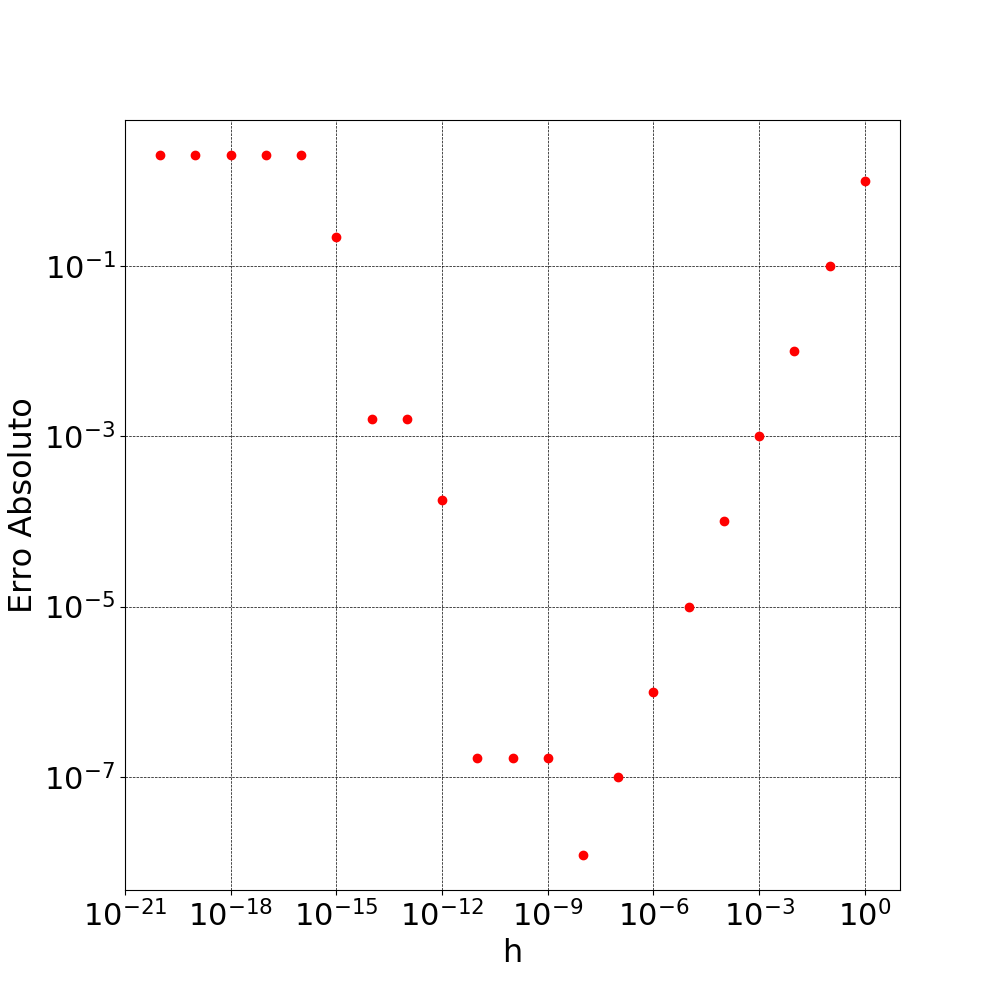
\includegraphics[width=\columnwidth]{erroh10.png} \\
	\caption{Erros absolutos de aproximações à primeira derivada da função quadrática em $x_0=1$ com $h=10^{-i}, i=1,\ldots,20$ em Python.}
  \label{figure2.1}
\end{figure}
Veja-se como nos cinco pontos em $h=[10^{-20},10^{-16}]$ o declive é nulo e $\Delta(h)\equiv2$. Deve-se a um erro de arredondamento. Tomemos o seguinte exemplo:
\begin{lstlisting}
 ln[1]: 2 + 10**(-18)
Out[1]:	2.0
\end{lstlisting}
Aproximadamente 16 dígitos são usados na mantissa para representar as casas decimais dos \textit{floats}. Como o resultado desta operação é $2.000000000000000001$ mas só é possível representar até à 16ª casa decimal, é arredondado para $2.0000000000000000$. O mesmo acontece para os outros valores de $h$ em $[10^{-20},10^{-16}]$.
\\
Para $h=[10^{-16},10^{-14}]$ vemos como o erro diminui. Seria de esperar o comportamento oposto. Esta diminuição pode ser justificada, mais uma vez, pelos erros de arredondamento. Veja-se o seguinte código:
\begin{lstlisting}
 ln[2]: ((1+10**(-15))**2 - 1)/(10**(-15)) < ((1+10**(-14))**2 - 1)/(10**(-14))
Out[2]: False
\end{lstlisting}
Esperar-se-ia que \texttt{Out[2]} fosse \texttt{True}, mas, devido aos arredondamentos tanto nas somas como nas divisões, acabamos por obter um resultado diferente no final ("Cancelamento Catastrófico"). Quanto menor $h$, maior o erro de arredondamento. Visto que o erro é um quociente de $h$, em $h=[10^{-16},10^{-9}]$, quanto menor $h$ maior $\Delta(h)$.\\
% Temos em $h=[10^{-11},10^{-9}]$ um declive nulo (os valores do erro para estes valores são iguais). Deve-se a dois fatores. O primeiro é o erro de arredondamento em cada uma das computações que faz com que os valores de $\Delta(h)$ estejam muito próximos. O segundo fator é sobre o armazenamento dos \textit{floats} no Python. Números muito próximos podem acabar por ser arredondados para o mesmo valor devido à incapacidade de representar todas as suas casas significativas.\\
% Atente-se que em $h=[10^{-16},10^{-9}]$ é onde os arredondamentos são tais que contrariam a natureza crescente da função erro. Em $h=[10^{-20},10^{-16}]$, o erro de arredondamento é tal que o resultado deixa de fazer sentido. Se $h=[10^{-16},10^{-9}]$ for a zona fronteira, $h=[10^{-20},10^{-16}]$ é a zona crítica.\\
O declive positivo em $h=[10^{-9},10^{0}]$ é o esperado: quanto menor $h$ menor o seu $\Delta(h)$ correspondente, tal como indica a definição da função erro. Isto pode indicar que a diferença de $10^{-9}$ na ordem dos números a serem computados no cálculo de cada erro não afeta o resultado (significativamente) quanto a arredondamentos ou representação de algarismos significativos.


\subsection{Erro absoluto em função de h (base 2)}
Consideremos, agora, o caso em que $h=2^{-i}, i=1,2,\ldots,60$. Os resultados obtidos podem ser visualizados na Figura~\ref{figure2.2}.\\
\begin{figure}[ht]
   \begin{center}
    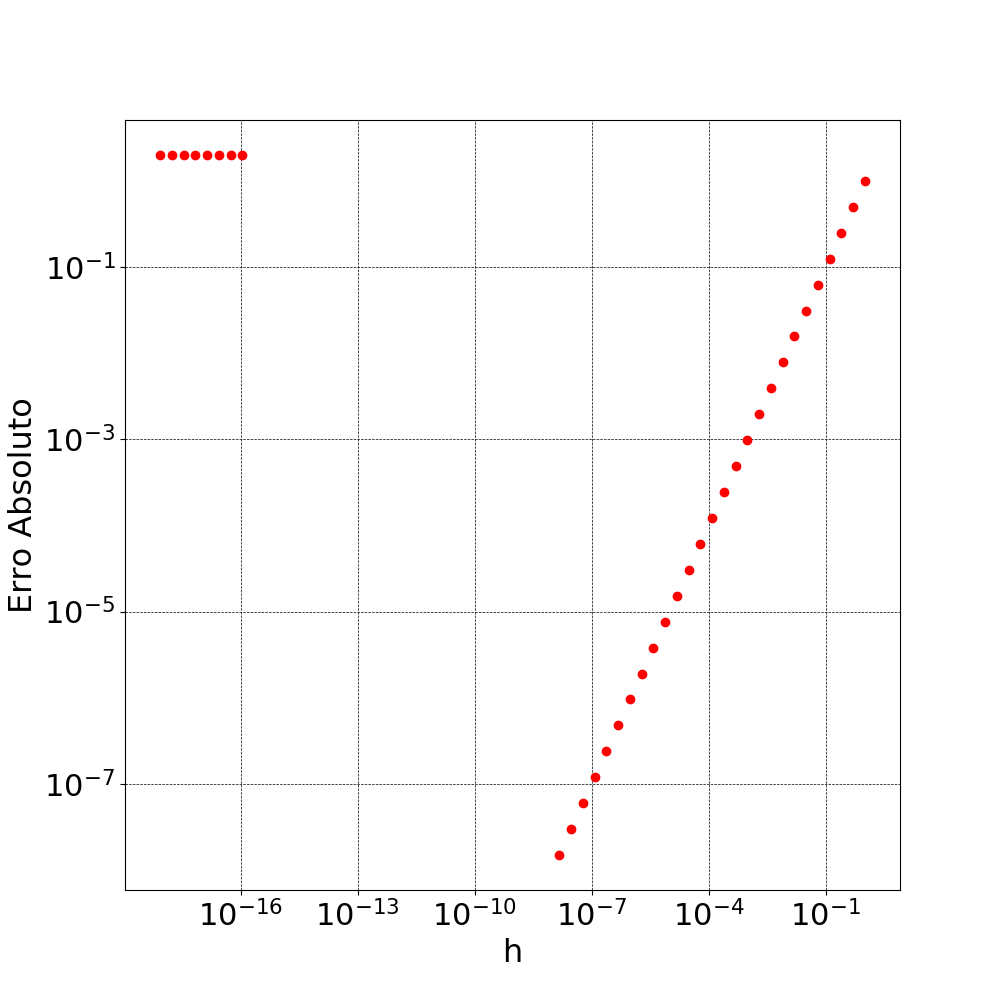
\includegraphics[width=\columnwidth]{erroh2.png} \\
	\caption{Erros absolutos de aproximações à primeira derivada da função quadrática em $x_0=1$ com $h=2^{-i}, i=1,2,\ldots,60$ em Python.}
  \label{figure2.2}
   \end{center}
\end{figure}
A parte inicial, $h=[10^{-19},10^{-16}]$, pode ser associada ao mesmo intervalo na Figura~\ref{figure2.1}.\\
Em $h=[10^{-16},10^{-8}]$, os valores do erro são nulos.
Para ilustrar o que acontece aqui, usemos como exemplo $\Delta(2^{-27})$. A máquina vai calcular
\begin{equation}
  \Delta(2^{-27})=2-\frac{(1+2^{-27})(1+2^{-27})-1}{2^{-27}}.
\end{equation}
% Em binário,
% \begin{equation}
%   \begin{split}
%     &\Delta(2^{-27})=\\
%     &=10-\frac{(1+0.000000000000000000000000001)(1+0.000000000000000000000000001)-1}{0.000000000000000000000000001}\\
%     &=10-\frac{1.00000000000000000000000001000000000000000000000000001}{0.000000000000000000000000001}\\
%     &=10-10\\
%     &=0, c.q.d\\
%   \end{split}
% \end{equation}
Fazendo $1+2^{-27}$ em binário vem $1+0.000000000000000000000000001=1.000000000000000000000000001$. A seguir multiplicamos este número por ele próprio e dá $1.00000000000000000000000001000000000000000000000$-$000001$, mas como a mantissa só tem capacidade para 52 casas decimais no binário, é arredondado para $1.00000000000000000000000001000000000000000000000$-$00000$.
Agora subtraímos $1.0$, donde resulta $0.00000000000000000000000001000000000000000000000$-$00000$.\\Num penúltimo passo, dividimos por $0.000000000000000000000000001$ e vem $10.0$.
O último passo é $10.0-10.0$ resultando em $\Delta(2^{-27})=0$, coincidindo com o valor no gráfico.
Isto acontece para os valores em $h=[2^{-27},2^{-52}]$ que correspondem ao intervalo $h=[10^{-16},10^{-9}]$ em base decimal. É este mesmo intervalo que, por contraste, apresenta o declive negativo na Figura~\ref{figure2.1}.\\
A partir daqui (intervalo $h=[10^{-8},10^{0}]$), o declive é positivo, como seria de esperar num intervalo real. Nesta ordem de grandeza os valores não são arredondados, porque não se atinge o limite de bits da mantissa.

\subsection{Erro absoluto usando Mathematica}
Nesta última subsecção, realizamos o mesmo estudo que na subsecção A, agora usando o software \textit{Wolfram Mathematica} que calcula o erro absoluto para todos os valores de $h$ que tem na memória dentro do intervalo. Veja-se Figura~\ref{figure2.3}. \\
\begin{figure}[ht]
   \begin{center}
    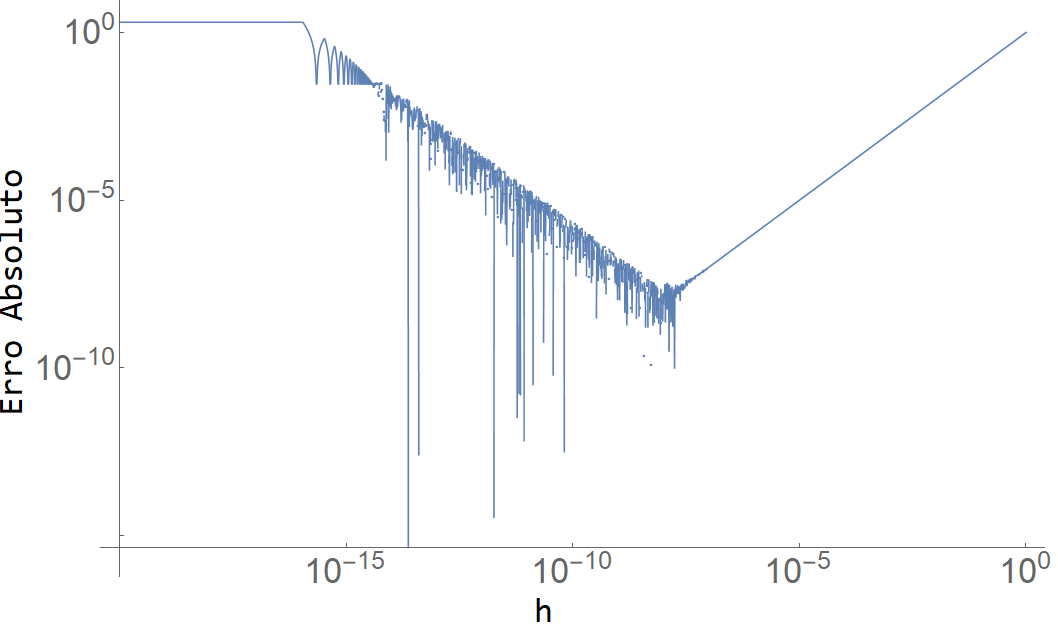
\includegraphics[width=\columnwidth]{erromathematica3.png} \\
	\caption{Erros absolutos de aproximações à primeira derivada da função quadrática em $x_0=1$ com $h=10^{-i}, i=1,2,\ldots,20$ com o software \textit{Wolfram Mathematica}.}
  \label{figure2.3}
   \end{center}
\end{figure}
Mais uma vez, obtemos aquela reta em $h=[10^{-20},10^{-16}]$ com declive nulo, devendo-se à mesma razão apontada na
subsecção A. \\
No intervalo $h=[10^{-16},10^{-8}]$, vemos como o valor do erro é predominantemente decrescente, com alguns valores muito mais baixos. Estes valores representam os $h$ de base $2$ em $h=[2^{-27},2^{-52}]$, pelas razões já mencionadas.\\
Já no intervalo $h=[10^{-8},1]$ vemos como se trata de uma reta de declive positivo $-$ mais uma vez, os arredondamentos não são relevantes.
\section{Conclusões}
Os resultados obtidos realçam a divergência do resultado de operações que envolvam \textit{floats} de ordens de grandeza inferior a $10^{-8}$.
\end{document}
